\documentclass[tikz,border=2pt]{standalone}
\usepackage{amsmath,amssymb}
\usepackage{tikz}
\usetikzlibrary{arrows.meta}

\begin{document}
% Aleph-null, the size of N: the even numbers form a proper subset of N, yet n -> 2n pairs
% them off with all of N, so they have the same cardinality aleph_0.
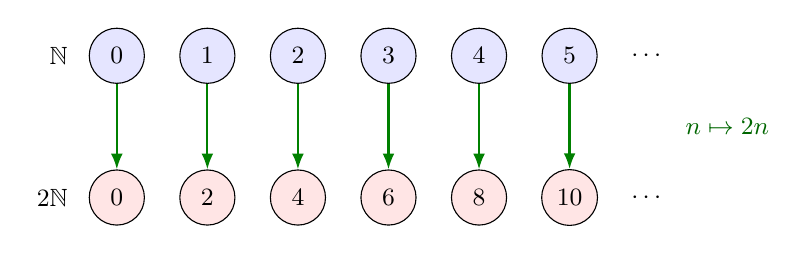
\begin{tikzpicture}[every node/.style={font=\small}, >={Latex[length=2mm]}]
	\foreach \n in {0,...,5} {
		\node[draw, circle, fill=blue!10, minimum size=7mm] (a\n) at (\n*1.15,0) {$\n$};
		\pgfmathtruncatemacro{\m}{2*\n}
		\node[draw, circle, fill=red!10, minimum size=7mm] (b\n) at (\n*1.15,-1.8) {$\m$};
		\draw[->, green!50!black, thick] (a\n) -- (b\n);
	}
	\node at (6.75,0) {$\cdots$};
	\node at (6.75,-1.8) {$\cdots$};
	\node[anchor=east] at (-0.5,0) {$\mathbb{N}$};
	\node[anchor=east] at (-0.5,-1.8) {$2\mathbb{N}$};
	\node[green!40!black, anchor=west] at (7.1,-0.9) {$n\mapsto2n$};
\end{tikzpicture}
\end{document}
